\quad 1.\quad Установка git, nodejs, npm и grunt.
\newline Для установки всего необходимого, нам нужно открыть терминал, нажав на его иконку.  

\begin{figure}[h]
		\centering
		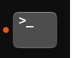
\includegraphics[width=0.1\linewidth]{VM/5.png}
\caption{Терминал.}
\label{ris:image}
\end{figure}

\quad Далее, для скачивания, необходимо ввести соответствующие строки кода:
\newline git – sudo apt install git
\newline nodejs – sudo apt install nodejs
\newline npm - sudo apt install npm
\newline grunt - sudo apt install grunt
\newline Чтобы удостовериться, что всё правильно скачалось, можно узнать версию данного продукта. Например: git –version

\quad 2.\quad  Регистрация на github.
\newline \quad Для регистрации на github нужно перейти по ссылке: : https://github.com/ и заполнить всю необходимую информацию о себе.

\quad     3. \quad Работа с репозиторием.
\newline \quad Переходим по ссылке: https://github.com/nickkolok/chas-ege/. Далее нажимаем на зелёную кнопку с надписью «Code», и копируем ссылку репозитория. Лучше сделать это сразу, потому что «Ubuntu» на «VirtualBox» может сильно нагружать компьютер, и открыть вкладку с браузером может быть проблематично из-за нагрузки. (Если возникли проблемы с копирование ссылки, то можно открыть браузер внутри «Ubuntu», перейти по ссылке и скопировать ссылку репозитория в нём.)

\begin{figure}[h]
		\centering
		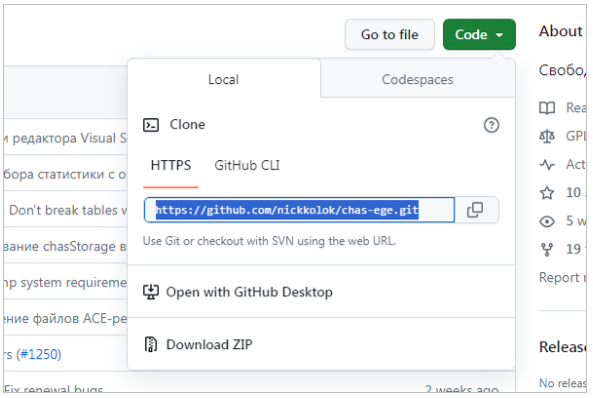
\includegraphics[width=0.65\linewidth]{VM/6.png}
\caption{Github. Ссылка на репозиторий.}
\label{ris:image}
\end{figure}

• Далее снова заходим в терминал и создаём папку на рабочем столе командой: mkdir <название папки>. Можете убедиться, что папка создана, с помощью команды: ls. Мы увидим все папки на рабочем столе, среди которых должна быть только что созданная.Затем заходим в папку командой: cd <название папки>, и клонируем себе репозиторий командой: git clone <ссылка на репозиторий >
  \newline   • Добавляем себе ссылку на основной репозиторий проекта с помощью команды: git remote add upstream <ссылка на репозиторий > и убеждаемся, что он подключился, командой: git fetch upstream 
   \newline  • Собираем проект командой: grunt. Важно выполнять эту команду в папке, в которую мы и склонировали репозиторий.
  \newline  • Открываем файл dist/sh/otladka.html в браузере командой: «open otladka.html», и запускаем любой шаблон, для проверки, в открывшемся окне.

\begin{figure}[h]
		\centering
		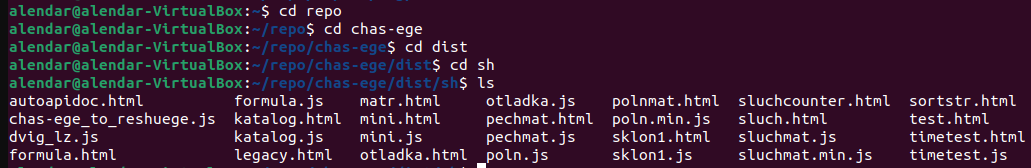
\includegraphics[width=1\linewidth]{VM/7.png}
\caption{Путь к файлу otladka.html.}
\label{ris:image}
\end{figure}

\quad 	4.\quad  Создание SSH ключа для возможности подключиться к удалённому репозиторию.
\newline \quad Для начала нужно проверить наличие ключа, введя следующие команды:
\newline «cd ~/.ssh»
\newline «ls»
\newline \quad Если файлов с названиями «id\_dsa» и «id\_dsa.pub» нет (открытый и приватный ключ), то можно создать их используя команду:
\newline  «ssh-keygen -o»
\newline \quad Далее нужно открыть содержимое файла dsa.pub командой:
\newline  «cat ~/.ssh/ id\_dsa.pub»
\newline \quad Далее добавили свой ключ себе в аккаунт на гитхабе, чтобы иметь возможность подключиться к удалённому репозиторию. А также прописали ещё одну команду, необходимую для подключения.

\begin{figure}[h]
		\centering
		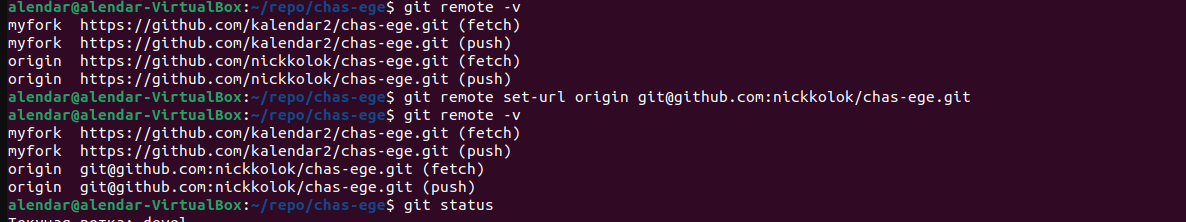
\includegraphics[width=1\linewidth]{VM/pod.png}
\caption{Подключению к удалённому репозиторию с помощью команды.}
\label{ris:image}
\end{figure}

\quad Перейдя в гитхабовский репозиторий "ЧАС-ЕГЭ", нужно нажать кнопочку "Fork" справа вверху.
\newline \quad Открыв «VirtualBox» и войдя в свою виртуальную машину, открыли терминал и перешли в папку с "Час ЕГЭ" с помошью команды cd git/chas-ege
\newline \quad Представление гиту выглядит следующим образом:
\newline git config --global user.name "Фамилия Имя"
\newline git config --global user.email "электронная почта пользователя"
Можно придать выводу гита красные и зелёные цвета с помощью команд:
git config --global color.ui true
Добавление своего форка на гитхаб в список удалённых репозиториев:
git remote add myfork git@ github.com:"GitgubNik"/chas-ege.git
где "GitgubNik" - ник пользователя на гитхабе. 

\quad Основные команды для создания и отправления изменений в удалённый репозиторий.
\\ \quad Переключение на основную ветку (devel):
\\ "git checkout devel"
\\ \quad Её обновление (В некоторых случаях применима также команда: git pull origin devel):
\\ "git fetch origin devel"
\\ \quad Создание новой ветки:
\\ "git checkout -b newtask-777"
\\ \quad Проверка изменений, а также самой ветки:
\\ "git status"
\\ \quad Добавление всех изменений:
\\ "git add ."
\\ \quad Добавление всех изменений:
\\ "git commit -m "Внесены изменения в файл ...""
\\ \quad Отправка изменений в удалённый репозиторий:
\\ "git push myfork newtask-777:myfork newtask-777:"
\\

\quad 	5.\quad  Игнорирование ненужных файлов и каталогов.
\newline \quad Для того, чтобы сообщить Git, какие файлы или каталоги нужно игнорировать , можно создать .gitignore файл.
\newline Для этого необходимо открыть Терминал и перейти к расположению репозитория Git. Далее создаётся файл для репозитория, с помощью команды «touch .gitignore».
\newline Если файл уже был отправлен в репозиторий, необходимо отменить отслеживание файла, прежде чем добавлено правило игнорирования, с помощью команды: «git rm —cached FILENAME».
\newline Файл не видим, как и все файлы с точкой в начале названия файла, но его можно увидеть с помощью команды ls -a. Зайдя в него, нужно записать путь к файлу или каталогу, который будет игнорироваться.

\begin{figure}[h]
		\centering
		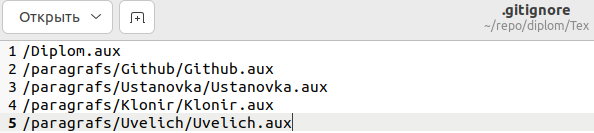
\includegraphics[width=0.8\linewidth]{VM/gitignore.png}
\caption{Файл .gitignore с списком файлов для игнорирования в нём.}
\label{ris:image}
\end{figure}

\quad Это не единственный способ задания игнорирования файла или каталога.
\newline Можно также сообщить Git всегда игнорировать определенные файлы во всех репозиториях на компьютере. Для этого, например, каталог нужно добавить в файл с именем ignore , расположенным внутри каталога ~/.config/git.

\quad Также можно вообще не создавать файл .gitignore. 
\newline Этот метод можно использовать для локально создаваемых файлов, которые не должны создавать другие пользователи. Для этого, используя текстовый редактор, нужно открыть файл, вызываемый .git/info/exclude в корневом каталоге репозитория Git.